\documentclass[../../../../main.tex]{subfiles}
\begin{document}

\begin{flushright}
\footnotesize\textit{【自動文字起こし・要確認】}
\end{flushright}

\noindent
[\textbf{解}] $l$ が $x$ 軸に一致し、$P(0, \sqrt{3}+1)$ となるよう $xy$ 平面をおく。

\begin{center}
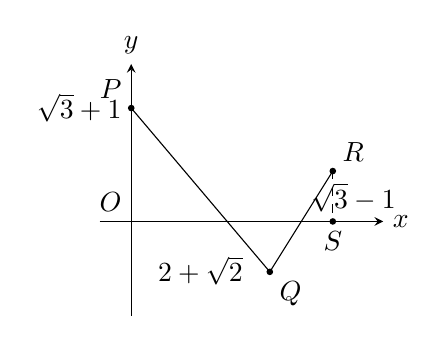
\begin{tikzpicture}[scale=0.8, >=stealth]
  \draw[->] (-0.5,0) -- (4.0,0) node[right] {$x$};
  \draw[->] (0,-1.5) -- (0,2.5) node[above] {$y$};
  \node[above left] at (0,0) {$O$};
  \fill (0,1.8) circle (1.5pt) node[above left] {$P$};
  \node[left] at (0,1.8) {$\sqrt{3}+1$};
  \fill (2.2,-0.8) circle (1.5pt) node[below right] {$Q$};
  \node[below] at (1.1,-0.4) {$2+\sqrt{2}$};
  \fill (3.2,0.8) circle (1.5pt) node[above right] {$R$};
  \node[above right] at (2.7,0.0) {$\sqrt{3}-1$};
  \fill (3.2,0) circle (1.5pt) node[below] {$S$};
  \draw (0,1.8) -- (2.2,-0.8) -- (3.2,0.8);
  \draw[dashed] (3.2,0.8) -- (3.2,0);
\end{tikzpicture}
\end{center}

\noindent
まず、$|PQ| = 2+\sqrt{2}$ より、$Q$ は半径 $2+\sqrt{2}$ の円
\[
x^2 + (y - \sqrt{3} - 1)^2 = (2 + \sqrt{2})^2
\]
上をうごく。同様に
\[
2+\sqrt{2} - (2-\sqrt{2}) \le |PR| \le (2+\sqrt{2}) + (2-\sqrt{2})
\]
\[
2\sqrt{2} \le |PR| \le 4 \quad (\text{間の値もすべてとる})
\]
だから、$R$ は、
\[
8 \le x^2 + (y - \sqrt{3} - 1)^2 \le 16
\]
上をうごく。このうち、$R$ と $x$ 軸との距離が $\sqrt{3}-1$ 以下である部分が求める領域で、右図斜線部（境界含む）。

\begin{center}
\begin{tikzpicture}[scale=0.8, >=stealth]
  % Axes
  \draw[->] (-4.5,0) -- (4.5,0) node[right] {$x$};
  \draw[->] (0,-2.5) -- (0,3.2) node[above] {$y$};
  \node[below left] at (0,0) {$0$};

  % Center P(0, sqrt(3)+1) ~ (0, 2.73)
  \coordinate (P) at (0, 2.732);
  
  % Outer arc R=4, Inner arc R=2*sqrt(2) ~ 2.828
  % Center at y = 2.732.
  % Outer circle passes through (0, -1.268) which is sqrt(3)-3.
  % Line y = sqrt(3)-1 ~ 0.732.
  % Line y = -sqrt(3)+1 ~ -0.732.

  % Shaded region bounded by outer arc, inner arc, y = sqrt(3)-1
  \begin{scope}
    \clip (-4.2, -2.0) rectangle (4.2, 0.732);
    \fill[pattern=north east lines, pattern color=gray] (P) circle (4);
    \fill[white] (P) circle (2.828);
  \end{scope}

  % Draw arcs
  \draw[thick] (P) ++(-60:4) arc (-60:-120:4);
  \draw[thick] (P) ++(-45:2.828) arc (-45:-135:2.828);
  
  % Horizontal boundary line y = sqrt(3)-1
  \draw[dashed] (-4.2, 0.732) -- (4.2, 0.732);
  \node[right] at (4.2, 0.732) {$\sqrt{3}-1$};

  % Labels on y-axis
  \fill (0,2.732) circle (1.5pt) node[left] {$\sqrt{3}+1$};
  \node[right] at (0,0.732) {$\sqrt{3}-1$};
  \node[right] at (0,-0.096) {$\sqrt{3}+1-2\sqrt{2}$};
  \node[right] at (0,-1.268) {$\sqrt{3}-3$};
  \node[left] at (-0.2,-0.732) {$-\sqrt{3}+1$};

  % Labels on x-axis
  \node[below] at (-4,0) {$-4$};
  \node[below] at (-2.828,0) {$-2\sqrt{2}$};
  \node[below] at (2.828,0) {$2\sqrt{2}$};
  \node[below] at (4,0) {$4$};

  % Angle labels
  \node at (-1.5,2.2) {$45^\circ$};
  \node at (1.8,2.5) {$60^\circ$};
  \node at (0.5,1.8) {$30^\circ$};
\end{tikzpicture}
\end{center}

\noindent
この面積 $S$ とする。右下図で、
\begin{align}
S = S_1 - S_2 \tag{1}
\end{align}
となり、
\begin{align*}
S_1 &= 2 \int_{2}^{2\sqrt{3}} \sqrt{16-x^2} \, dx \\
&= 2 \int_{\frac{\pi}{6}}^{\frac{\pi}{3}} 16 \cos^2 \theta \, d\theta \\
&= 16 \left[ \theta + \frac{1}{2} \sin 2\theta \right]_{\pi/6}^{\pi/3} \\
&= \frac{8}{3}\pi
\end{align*}

\begin{center}
\begin{tikzpicture}[scale=0.7, >=stealth]
  % S1 diagram
  \begin{scope}[shift={(0,0)}]
    \draw (-3,0) -- (3,0);
    \draw (0,-1.5) -- (0,0);
    \draw (-2.5,0) arc (-150:-30:2.89);
    \fill[pattern=north east lines, pattern color=gray] (-2.5,0) arc (-150:-30:2.89) -- cycle;
    \node at (0,-0.8) {$S_1$};
    \node[above] at (-2.5,0) {$-2\sqrt{3}$};
    \node[above] at (2.5,0) {$2\sqrt{3}$};
    \node at (0, 0.4) {$30^\circ$};
    \node at (-1.5, 0.4) {$4$};
    \node at (1.5, 0.4) {$4$};
  \end{scope}

  % S2 diagram
  \begin{scope}[shift={(7,0)}]
    \draw (-2.5,0) -- (2.5,0);
    \draw (0,-1.5) -- (0,0);
    \draw (-2,0) arc (-135:-45:2.828);
    \fill[pattern=north east lines, pattern color=gray] (-2,0) arc (-135:-45:2.828) -- cycle;
    \node at (0,-0.8) {$S_2$};
    \node[above] at (-2,0) {$-2\sqrt{2}$};
    \node[above] at (2,0) {$2\sqrt{2}$};
    \node at (1.2, 0.4) {$45^\circ$};
  \end{scope}
\end{tikzpicture}
\end{center}

\begin{align*}
S_2 &= (\text{扇形}) - (\text{三角形}) \\
&= \frac{1}{2} \cdot \frac{\pi}{2} \cdot (2\sqrt{2})^2 - \frac{1}{2} \cdot 2 \cdot 2 \cdot 2 \\
&= 2\pi - 4
\end{align*}
(1)に代入して
\[
S = 4 + \frac{2}{3}\pi
\]

\newpage

\end{document}
